\section{Results}

\subsection{Description of the Artefact}
The end product is a software application: a working prototype (an instantiation, in Design Science Research terms) that turns the Reachy Mini into a CPU-only activity monitor that answers what it sees with its own body.
It consists of three parts: a layered software architecture that runs the same recognition code in simulation and on the robot, recognition models exported as NumPy-only files, and robot applications built on both.
It addresses the requirements of the software requirements specification (SRS) attached to this article (Section~3.1).

\begin{figure}[htbp]
  \centering
  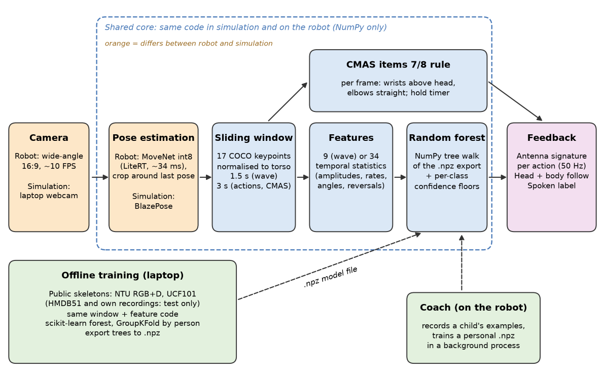
\includegraphics[width=\linewidth]{figures/pipeline_architecture.png}
  \caption{Pipeline Architecture.}
  \label{fig:pipeline}
\end{figure}

Figure~\ref{fig:pipeline} represents the artefact's pipeline.
Everything inside the dashed line is the same code in simulation and on the robot; only the camera and the pose estimator differ.
Models are trained offline, or by the coach on the robot, and loaded as \texttt{.npz} files.

The pipeline works in such way that a camera frame goes to a pose estimator that returns 17 COCO keypoints: MoveNet Lightning int8 on the robot, BlazePose on the laptop webcam in simulation.
The keypoints enter a sliding window, are normalised to the torso and summarised as temporal features.
A random forest, evaluated by a NumPy-only tree walk, classifies every window, and a per-class confidence floor turns uncertain windows into \emph{none}.
Each detection drives the feedback: a distinct antenna signature per action, rendered at 50~Hz independently of the 10~FPS vision loop, head and body following that keeps the person in view, and an optional spoken label.

As for architecture and organization, the code is organised by where it must run: a shared core (pose backends, features, models, feedback), robot applications, simulation tools for MuJoCo and a webcam, and training tools, which are the only part that needs scikit-learn.
Dependencies point only into the core, so one model file and one feature implementation serve both environments, and training and inference cannot drift apart.

For the final application, the robot runs action recognition (the six classes, or the CMAS items of Section~4.6), wave recognition, head and body tracking, and a coach for children.
The coach guides a child through about 4.5 minutes of recording (squats, arm raises, side bends), trains a personal model on the robot's own CPU while the head keeps following, and then runs a workout with that model.
A preflight tool brings the robot into a known state before every application.

Table~\ref{tab:decisions} links the main decisions to the requirement or insight behind them.

\begin{table}[htbp]
  \centering
  \caption{Origin of the main design decisions.}
  \label{tab:decisions}
  \rowcolors{2}{white}{white}
  \begin{tabular}{|p{0.44\textwidth}|p{0.44\textwidth}|}
    \hline
    \rowcolor{gray!20}\textbf{Origin} & \textbf{Decision} \\
    \hline
    Requirement: local processing on a CPU without GPU & MoveNet int8 for pose; forests exported to NumPy instead of a deep skeleton network \\
    \hline
    Requirement: privacy of child users & Only keypoints are stored; children's recordings and models stay on the robot \\
    \hline
    Grounding: windowed data leaks between splits & Every score from GroupKFold by person \\
    \hline
    Grounding: public datasets may not transfer to a room & Robot and room recordings kept as external test sets only \\
    \hline
    Design cycle: BlazePose cannot run on the robot's CPU (its binary needs AES instructions) & Pose backend made swappable behind one interface \\
    \hline
    Design cycle: a table-mounted camera often sees the person waist-up & Training windows also built with hips and legs removed \\
    \hline
    Design cycle: letterboxing the 16:9 wide-angle frame left the person a few dozen pixels tall & Pose crop centred on the previous pose; person detected in 72\% of frames instead of 52\% \\
    \hline
    Design cycle: scikit-learn inference cost ${\sim}33$~ms per window on the robot & Trees exported to \texttt{.npz} and walked in NumPy \\
    \hline
    Design cycle: the robot often boots asleep, motors off, camera released & Preflight with automatic fix \\
    \hline
  \end{tabular}
\end{table}

\subsection{Pose-Model Performance}
The benchmark compared BlazePose, MoViNet-A0, TSM-MobileNetV2, ViTPose and MoveNet as candidates for the perception pipeline.
MoveNet Lightning int8 reached 23.80~FPS in the inference benchmark, with a mean pose-inference time of approximately 34~ms on the Reachy Mini; in the complete application the camera, at about 10~FPS, sets the rate (Section~4.5).
This was the most suitable result for the CPU-only target, and the model produces the COCO-17 keypoints the recognition code expects.
Cropping each frame around the previous pose, instead of letterboxing the whole wide-angle frame, raised the share of robot frames with a detected person from 52\% to 72\%.
On a replay of a laptop recording with the robot's aspect ratio, it raised the mean keypoint confidence from 0.48 to 0.68.

\subsection{CMAS Items}
In CMAS mode the prototype recognises that four CMAS items were performed; it does not score them.
Items~12 (chair rise) and~14 (pick-up) are classified by a three-class forest (none, chair rise, pick-up) trained on NTU RGB+D alone (actions \enquote{standing up} and \enquote{pick up}).
Items~7 and~8 (arms straight above the head, and for how long) use a geometric rule on single frames, because a held posture has no movement for a window to learn.
Item~13 (stool step) was left out: no public dataset contains it and none was recorded.
